\section{Domain model}
\begin{comment}
Give a high level view overview of the application using a UML diagram.
\end{comment}
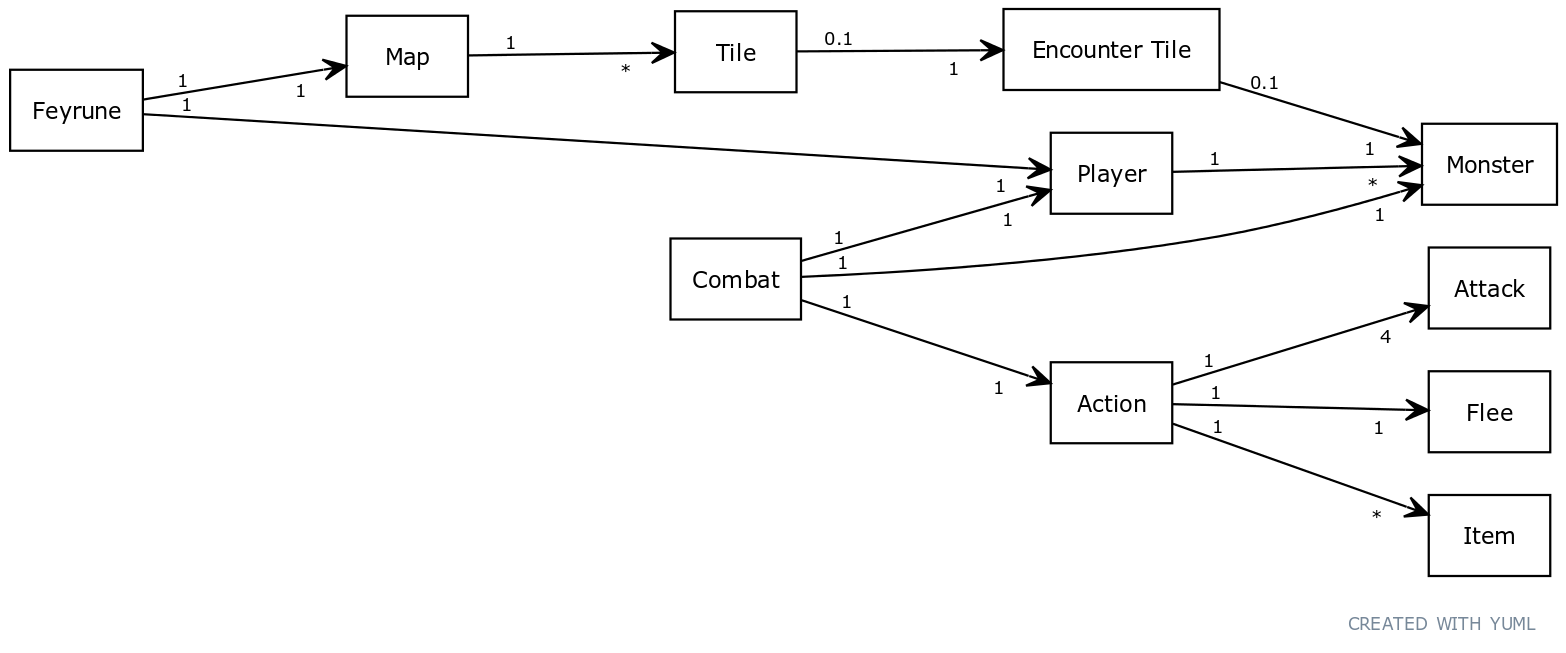
\includegraphics[width=\textwidth]{images/domain_model.png}

\subsection{Class responsibilities}
\begin{comment}
Explanation of responsibilities of classes in diagram.
\end{comment}
\begin{itemize}
    \item Feyrune
    \subitem Feyrune is the name of our game/ application and is the main program.
    \item Map
    \subitem Map is a tiled map that has information about all that the can be seen and explored in the world
    \item Tile
    \subitem A tile is a small part of the map that has information about what that specific tile, ex graphics, collision and encounter
    \item Encounter Tile
    \subitem The Encounter Tile can with chance start a combat with generates a monster and takes information about the players owned monsters
    \item Player
    \subitem The Player has a collection of monsters, some items and a position on the Map. The player is also what you as a user can control.
    \item Combat
    \subitem The combat has one enemy and a players monster that fight until death or someone flees. There are a number of actions that both the enemy monster and the players monster can do
    \item Action
    \subitem An action is what you or the enemy can do in a combat
    \item Monster
    \subitem A monster is a creature with stats and is the cornerstone of this application
    \item Attack
    \subitem All monsters can have one to four different attacks that have different effects on the combat or simply do different amounts of damage
    \item Flee
    \subitem The flee action lets you have a chance to leave the combat without having to fight until death
    \item Item
    \subitem An item is a separate action from an attack that can have different effect on the combat
\end{itemize}